\chapter{Návrh aplikace}
Před vývojem aplikace je klíčové dobře promyslet veškeré aspekty, které následně ovlivňují návrh řešení. V~tomto konkrétním případě jde o~tři otázky. Jak bude server data přijímat? Kam je bude ukládat? Jak se budou data zobrazovat uživateli? Vše ostatní je svým způsobem \uv{pouze} kód, který tento návrh umožňuje. Samotný kód je ovšem neméně důležitý. Špatně naprogramovaná aplikace může znamenat narůstající vytváření technického dluhu \cite{techdebt}, který povede k~nepřehledné a špatně udržovatelné aplikaci. Následující sekce postupně poodhalují návrhy jednotlivých částí aplikace a myšlenky, které k~tomuto návrhu vedly.

%%%%%%%%%%%%%%%%%%%%%%%%%%%%%%%%%%%%%%%%%%%%%%%%%%

\section{Přenos a ukládání dat z~meteostanic}
Ať už se jedná o~webovou kameru nebo o~meteorologickou stanici, aplikace musí nějak data získat a uložit je pro pozdější zpracování. Existují v~zásadě dva přístupy, jak data získávat. Aplikace může data od koncových zařízení sbírat, nebo je může přijímat. Jedná se o~zcela protichůdné procesy. Zatímco při sbírání musí aplikace vynaložit nemalé úsilí pro dotazování se na nová data, tak při naslouchání pouze čeká až nová data přijdou a ty následně uloží. Proto se tento druhý přístup používá v~praxi mnohem častěji a stejně je tomu i v~této práci.

\begin{figure}[h]
    \centering
	\makebox[\textwidth]{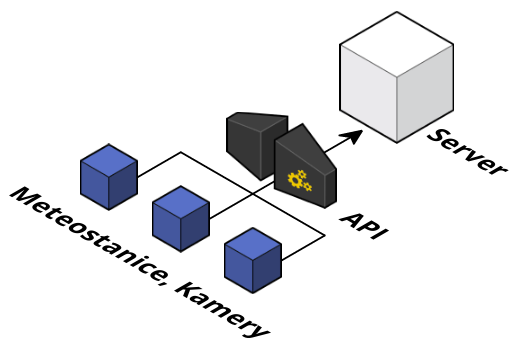
\includegraphics[width=0.8\textwidth]{img/zakladni-navrh-crop.png}}
	\caption{Základní návrh aplikace}
	\small zdroj: Vlastní tvorba - \url{https://cloudcraft.co/}
	\label{fig:zakladniNavrh}
\end{figure}

Aplikace tedy funguje stejně jako je znázorněno na obrázku \ref{fig:zakladniNavrh} - jako posluchač. Koncová zařízení odesílají na server požadavky a server je přijímá a ukládá pro pozdější zpracování. Každé zařízení však komunikuje svým originálním způsobem. Neexistuje jednotný formát dat, jsou dány pouze komunikační protokoly.

Aby se předešlo tomu, že server bude muset vědět jak funguje každý zdroj dat, který existuje, tak je vhodnější vytvořit jednotné veřejné API. Toto API bude dostupné pro každého, kdo chce se serverem komunikovat a důležité je, že není závislé na typu zařízení. Z~toho plyne, že se každé zařízení musí podřídit a komunikovat předem daným způsobem. Obrovskou výhodou tohoto přístupu je úleva zodpovědnosti serveru. Nemusí totiž vědět odkud data pocházejí, protože jsou pořád stejná. Místo toho se může soustředit na vykonávání své hlavní činnosti - zpracovávání a ukládání jednotného formátu dat. V~celém systému se tak stává zdrojem pravdy.

Zůstává však otázka, jak z~meteostanice tato data odeslat na API? Ně\-kte\-ré meteostanice odesílají UDP datagramy se svým vlastním formátem dat, jiné zase fungují jen přes sériovou linku (a tedy po síti neodesílají nic) a třeba takové kamery streamují obraz přes RTSP protokol. Ani jeden zmíněný způsob není s~API kompatibilní. Proto je nutné představit celému API vrstu, která kompatibilitu zajistí. Ta může být součástí infrastruktury, nesmí však být součástí serveru. Tuto myšlenku zachycuje lépe obrázek \ref{fig:zakladniNavrh2}. Veškerá data z~meteostanice, která neumí komunikovat s~API přímo, musí nejdříve projít programem, který zajistí kompatibilitu s~API. Tento program může využívat více meteostanic, pokud jsou stejného typu. Speciální případ potom tvoří kamera, kde je nutné nejdříve zpracovat stream dat a serveru předat pouze adresu tohoto nově vytvořeného a upraveného streamu. Server potom tento stream nabízí k~dispozici pro prohlížeč, ale sám se nestará o~jeho zpracování (viz popis streamování videa z~první kapitoly).

\begin{figure}[h]
    \centering
	\makebox[\textwidth]{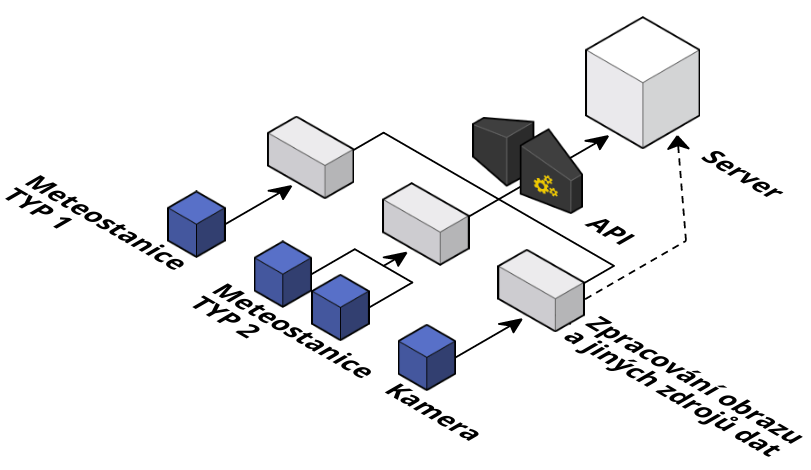
\includegraphics[width=\textwidth]{img/zakladni-navrh-rozsireny-crop.png}}
	\caption{Základní návrh aplikace s~mezivrstvou pro API}
	\small zdroj: Vlastní tvorba - \url{https://cloudcraft.co/}
	\label{fig:zakladniNavrh2}
\end{figure}

Server následně ukládá data do databáze, kterou v~tomto případě zastupuje PostgreSQL \cite{postgresql}. Volba databáze není ničím ovlivněna. Bylo možné vybrat téměř libovolnou relační databázi (například MySQL). V~této práci se však hojně využívá UUID identifikátorů a PostgreSQL je na rozdíl od jiných databází přímo podporuje. Toto je pouze výhoda zvolené databáze, nikoliv důvod zvolení databáze.

%%%%%%%%%%%%%%%%%%%%%%%%%%%%%%%%%%%%%%%%%%%%%%%%%%

\section{Architektura serverové části aplikace}
U~jakékoliv webové aplikace se vždy řeší stejný problém. Klient (webový prohlížeč, CLI) pošle požadavek na server (data z~meteostanice), server předá tento požadavek aplikaci, ta na něj náležitě zareaguje a odešle klientovi zpět odpověď. Tento cyklus se neustále opakuje a napsat se dá téměř jakkoliv. Aby měl však program nějakou hodnotu, je nutné věnovat se dostatečně dlouho jeho návrhu. Nejde tedy pouze o~napsání několika řádek kódu. Jde o~hledání správného řešení.

Podívejme se detailněji na celou cestu od webového prohlížeče přes server zpět k~prohlížeči. Otevřením stránky \url{http://example.com/} webový pro\-hlí\-žeč odesílá GET požadavek.

\begin{minted}{text}
GET / HTTP/1.1
Host: example.com
Connection: keep-alive
Cache-Control: no-cache
Upgrade-Insecure-Requests: 1
User-Agent: Chrome/56.0.2924.87
Accept: text/html,application/xhtml+xml,application/xml;q=0.9
Accept-Encoding: gzip, deflate, sdch
Accept-Language: en-US,en;q=0.8
\end{minted}

Server tento pořadavek přijímá na portu číslo 80 a předává jej běžící službě, která na základě tohoto požadavku spouští aplikaci (v~případě této práce PHP 7.1). Stejná cesta funguje i pro odpověď, pouze opačným směrem. Vše ostatní se odehrává v~rámci aplikace. Bude proto zajímavější podívat se, co se děje právě zde (popisováno na vytvořené aplikaci v~této DP práci).

Webový server je nastaven tak, aby vždy posílal požadavek na soubor \texttt{www/index.php} v~adresářové struktuře aplikace. Zde se vytvoří DIC kontejner a aplikace se spustí:

%startinline needed only for PHP without <?php
\begin{minted}[startinline]{php}
<?php declare(strict_types = 1);

/** @var Nette\DI\Container $container */
$container = require __DIR__ . '/../bootstrap.php';
$container->getByType(Nette\Application\Application::class)
          ->run();
\end{minted}
%$ (highlighter terminator)

Toto se odehrává při každém požadavku. Vnitřně se aplikace podívá na URL adresu a podle nastavení dokáže přiřadit konkrétní GET požadavek konkrétnímu kontroleru. Jakmile aplikace dojde až do kontroleru, je čas vykonat nějakou operaci. V~tomto jednoduchém případě by se jednalo pouze o~vykreslení šablony a odeslání zpět. Představme si ale případ, kde je potřeba uložit něco do databáze.

Nebyl by žádný problém začít vykonávat tuto operaci přímo v~kontroleru. Je to ten nejjednodušší přístup, ale má svá zrádná úskalí. Úkolem kontroleru je delegovat práci někam dál. Na nějaké místo v~aplikaci, které je na tento úkol specializované a provádí pouze tuto jednu věc. To je velmi důležitý princip (SRP). Pokud dokážeme vytvářet kousky aplikace tak, že jsou samostatné a na jednu věc specializované, bude jednoduché je udržovat a automaticky testovat. Navíc to přispívá přehlednosti a kontrole nad programem.

V~této práci je kromě SRP použit ještě koncept kontextů. Aplikace je rozdělena na menší logické celky (kontexty), které fungují jako samostatné zapouzdřejné jednotky. Pokud potřebuje nějaký kontroler vykonat např. vložení do databáze jako v~předchozím příkladu, tak pouze na programovou sběrnici odešle příkaz, který se automaticky odešle do správného kontextu a ten jej zpracuje.

%startinline needed only for PHP without <?php
\begin{minted}[startinline]{php}
$commandBus->dispatch(new RegisterNewUser(
  'username',
  '53cr3tPa55w0rd'
));
\end{minted}
%$ (highlighter terminator)

\texttt{RegisterNewUser} je pouze obyčejný value objekt \cite{valueobject}, který zapouzdřuje přenášená data. Po spuštění se nevrací žádná hodnota a předpokládá se, že příkaz proběhne v~pořádku. Zároveň je takto zajištěna databázová transakce i kontrola oprávnění (opět uvnitř kontextu).

\subsection{Hexagonální architektura}
Je dobrý nápad oddělovat jednotlivé kontexty uvnitř aplikace. Jak toho ale dosáhnout bez využití mikroslužeb jen na úrovni společného kódu? Odpovědí může být právě hexagonální architektura. Místo toho, aby mohl v~kódu kdokoliv dělat cokoliv, tak stanovíme hranice pomocí příkazů, které se spouští díky sběrnici. Takto vypadá malý výřez adresářové struktury v~aplikaci:

\vspace{1em}
\dirtree{%
.1 src/.
.2 Authentication\DTcomment{řízení oprávnění}.
.3 Application\DTcomment{I/O porty balíčku}.
.3 DomainModel\DTcomment{doménový model}.
.3 Infrastructure\DTcomment{implementační detaily doménového modelu}.
.2 Devices\DTcomment{zařízení (meteostanice, kamery, apod.)}.
.3 Application.
.3 DomainModel.
.3 Infrastructure.
}
\vspace{1em}

\texttt{Authentication} i \texttt{Devices} jsou kontexty, které se starají o~uživatelské účty včetně oprávnění uživatelů resp. o~zařízení (meteostanice, webkamery, apod.). Každý tento kontext obsahuje tři hlavní části: \texttt{Application}, \texttt{DomainModel} a \texttt{Infrastructure}.

Část \texttt{Application} obsahuje již dříve zmíněné příkazy (commandy) a jejich obsluhu. S~kontextem je tedy možné komunikovat pouze prostřednictvím této aplikační vrstvy\footnote{Ve skutečnosti je možné programově zasáhnout i přímo do kontextu. Tomu bohužel nejde nijak zabránit, protože by aplikace nešla testovat. Je tedy třeba dodržovat určitá pravidla. Toto je jedno z~nich.}.

\texttt{DomainModel} potom obsahuje veškerou logiku, která \textbf{není závislá na implementačních detailech}. Tato poslední poznámka je pro dobrý návrh klíčová. Model jednoduše nesmí vědět o~tom, že existuje nějaká databáze, do které se data ukládají. Nesmí vědět, že existuje nějaký konkrétní typ meteorologické stanice. Může ale vědět, že existuje pojem meteorologické stanice a s~ním pracovat. Pokud dokážeme odlišit tento rozdíl, pak bude doménový model fungovat pro jakoukoliv meteostanici a nemusíme řešit implementační detaily. Dosáhneme toho využitím rozhraní v~PHP \cite{php:interfaces}.

A~konečně se dostáváme k~\texttt{Infrastructure}. Právě zde jsou umístěny jednotlivé implementační detaily. Detaily typu jakou databázi aplikace používá, jak se do ní data ukládají, popř. jak se aplikace napojuje na CLI nebo prezentační část.

Hexagonální architektura se ve svém původním znění používá spíše pro vytváření kontextů u~jednotlivých mikroslužeb pro složitější návrhy. To však neznamená, že nelze stejné postupy aplikovat v~rámci jednoho kódu a do\-dr\-žo\-vat stejná pravidla. Jedna z~velkých předností hexagonálního návrhu je možnost odložit rozhodnutí. Pokud totiž vytváříme aplikaci, tak by mělo být jedno do jaké databáze se následně data uloží. Můžeme bez větších problémů navrhnout celý doménový model a až na samotném konci se rozhodnout a zvolit tu správnou databázi. Databáze je totiž jen implementační detail \cite{screamingArchitecture}\footnote{V praxi se ukazuje, že je rozumné mít na paměti s~jakou databází se pracuje a využívat toho. Pro většinu aplikací však tato znalost nepřináší větší výhody než odstínění se od této skutečnosti.}.

\subsection{Konkrétní příklad ovládání kontextu}
Hexagonální architekturu si lze představit jako cibuli s~vrstvou slupek. Pokud se chceme dostat k~samotnému jádru, musíme projít přes několik vrstev (slupek). Samotné jádro (doménový model) neví o~implementační detailech, ty jsou ve vyšší vrstvě obalující jádro. Tato vrstva tak tvoří prostředníka mezi konkrétní technologií a nezávislým jádrem programu, jako je znázorněno na obrázku \ref{fig:hex1}. Z~levé strany přicházejí požadavky z~webového prohlížeče, popř. z~konzole nebo API, a z~pravé strany probíhá komunikace s~databází.

\begin{figure}[h]
    \centering
	\makebox[\textwidth]{\includegraphics[width=0.8\textwidth]{img/hexagonal-1.png}}
	\caption{Hexagonální architektura}
	\label{fig:hex1}
\end{figure}

Z~toho je vidět, že každý tento vstup má vlastní komunikační protokol, a proto je znázorněn v~jiné části šestiúhelníku. Úkolem infrastrukturní vrstvy je tyto požadavky přeložit a komunikovat s~jádrem\footnote{V anglických textech se vstupům říká porty a překlady požadavků probíhají pomocí adaptérů. Např. požadavek z~webového prohlížeče přichází na HTTP port, kde adapterem je kontroler.}. Prakticky to probíhá tak, že požadavek z~webového prohlížeče přichází jako HTTP zpráva do kontroleru v~aplikaci. Kontroler pouze vytvoří jednoduchý objekt reprezentující požadavek a odešle jej jako příkaz jádru. V~tomto případě vytvoření nové meteostanice:

%startinline needed only for PHP without <?php
\begin{minted}[startinline]{php}
$commandBus->dispatch(new CreateWeatherStation(
  'Weather Station Name',
  UserId::createFromString($userId) // UUID
));
\end{minted}
%$ (highlighter terminator)

Takto odeslaný příkaz jádru je již zbavený informace o~původní technologii. Díky tomu je možné použít stejný princip pro přicházející komunikaci z~jakéhokoliv zdroje. Jde pouze o~vytvoření objektu \texttt{CreateWeatherStation} a odeslání na sběrnici příkazů. Samotné vytváření objektu je právě záležitost infrastrukturní vrstvy. Je důležité uvědomit si, že komunikace probíhá pouze od vyšších vrstev k~nizším. Tak je zajištěno, že jádro neví o~infrastruktuře. Problém ale nastává při komunikaci s~databází. Pokud mají požadavky putovat pouze směrem do středu, jak může jádro něco ukládat do databáze, pokud o~databázi nesmí vědět?

První naivní postup by byl v~jádru zavolat nějaký objekt, který by rovnou uložil data do databáze. Říkejme mu repozitář \cite{repository}. Tento repozitář by však musel vědět, že se používá PostgreSQL a tedy jádro volá část programu obsahující implementační detaily. To je nežádoucí. Místo toho je mnohem vhodnější vyžadovat rozhraní \cite{php:interfaces}, které neobsahuje informace o~databázi, ale pouze dává k~dispozici jakýsi předpis toho, co bude konkrétní implementace umět. Tato myšlenka je zachycena na obrázku \ref{fig:hex2} pomocí UML diagramu.

\begin{figure}[h]
    \centering
	\makebox[\textwidth]{\includegraphics[width=\textwidth]{img/hexagonal-uml.png}}
	\caption{UML diagram konkrétních implementací repozitáře}
	\label{fig:hex2}
\end{figure}

K~dispozici je jedno rozhraní \texttt{IAllCamerasRepository}, které je vy\-u\-ží\-vá\-no jádrem. Vedle rozhraní existují i konkrétní implementace, které již vědí o~technologii. Jádro vyžaduje rozhraní, ale DIC se postará o~to, aby bylo toto rozhraní nahrazeno konkrétní implementací. Efekt je pak takový, že v~jádru je možné programovat technologicky nezávisle, ale program bude fungovat např. díky PostgreSQL. Tomuto postupu se říká Inversion of Control \cite{ioc}.

Využívání rozhraní má ještě jednu obrovskou výhodu. Při automatickém testování může být nežádoucí pracovat přímo s~databází z~důvodu rychlosti. Testy musí být rychlé. Proto je možné místo PostgreSQL implementace použít implementaci, která využívá pouze dočasnou paměť. Testy se tak násobně zrychlí. Takové testování je naprosto v~pořádku pokud nechceme testovat funkčnost repozitáře, ale nějakou třídu, která jej využívá.

\subsection{Kompletní adresářová struktura}
Celá hlavní aplikace je v~této práci postavena s~využitím Nette Frameworku \cite{netteorg}. Celá adresářová struktura je znázorněna v~následující části. Je zde vidět dříve popisované jádro aplikace ve složce \texttt{src}.

\vspace{1em}
\dirtree{%
.1 /.
.2 bin.
.3 console\DTcomment{spouštěč CLI}.
.2 config.
.3 config.local.neon\DTcomment{lokální konfigurační soubor}.
.3 config.neon\DTcomment{obecný konfigurační soubor}.
.2 extensions\DTcomment{implementace služeb třetích stran}.
.2 migrations\DTcomment{databázové migrace}.
.3 basic-data\DTcomment{základní data}.
.3 dummy-data\DTcomment{testovací data}.
.3 structures\DTcomment{základní struktury}.
.2 src.
.3 Authentication.
.3 Devices.
.3 ....
.2 tests\DTcomment{testy aplikace}.
.2 var\DTcomment{logy a cache}.
.2 vendor\DTcomment{služby třetích stran}.
.2 www\DTcomment{veřejná složka}.
.3 index.php\DTcomment{vstupní bod aplikace}.
.2 bootstrap.php\DTcomment{vytváří DIC kontejner}.
.2 composer.json/.lock\DTcomment{definice závislostí třetích stran}.
}
\vspace{1em}

Vstupním bodem je soubor \texttt{www/index.php}. Tímto souborem projde ve\-ške\-rá HTTP komunikace, která je následně zpracovávána v~jednom z~kontextů ve složce \texttt{src}. Komunikace s~aplikací prostřednictvím CLI zase probíhá přes \texttt{bin/console}:

\begin{minted}{text}
$ bin/console dbal:run-sql "SELECT * FROM user_accounts"
array(1) {
  [0]=>
  array(3) {
    ["id"]=>
    string(36) "00000000-0000-0000-0000-000000000001"
    ["password_hash"]=>
    string(60) "$2y$10$8nJLFVEGIFRnSyb5vjukQ/tJ/V4Yupa3O..."
    ["username"]=>
    string(4) "test"
  }
}
\end{minted}

Soubor \texttt{index.php} dělá pouze to, že vytváří DI kontejner (DIC), který se stará o~správné složení objektového grafu a obstárávání závislostí napříč aplikací. Následně z~tohoto kontejneru získá aplikační službu, která se stará o~běh aplikace. Význam ostatních částí je zřejmý z~popisků, jen testy a migrace jsou rozebrány ve zvláštních částech, které následují.

\subsection{Testování aplikace a CI provoz}
Napsání kódu je jen polovina problému. Každá správná aplikace musí mít automatické testy. Testy mají jediný význam. Kontrolují, jestli dříve napsaný kód funguje tak, jak bylo původně zamýšleno. Mnohdy se význam testů překrucuje a říká se, že díky testům neobsahuje aplikace chyby. To není správně. Díky testům neobsahuje pouze chyby, o~kterých již víme - jinak chyby stále obsahuje.

U~takových testů je důležité jejich neustálé spouštění. Každá nová řádka, dokonce i nový znak v~programu může způsobit nefunkčnost nějaké části aplikace a není v~lidských silách vždy kontrolovat vše. Spuštění testů se v~této aplikaci provádí pomocí příkazu \texttt{tests/run}:

\definecolor{testerGreen}{HTML}{00A220}
\begin{minted}[escapeinside=@@]{text}
$ tests/run
TESTBENCH edition
 _____ ___  ___ _____ ___  ___
|_   _/ __)( __/_   _/ __)| _ )
  |_| \___ /___) |_| \___ |_|_\  v2.0.x

PHP 7.1.1 (cli) | php | 8 threads | /tests/bootstrap.php

  @\textcolor{testerGreen}{[OK] GraphQL/DomainModel/DateTimeTypeTest.phpt}@
  @\textcolor{testerGreen}{[OK] DI/Nette/ExtensionEnumTest.phpt}@
  @\textcolor{testerGreen}{[OK] DomainModel/Humidity/RelativeHumidityTest.phpt}@
  @\textcolor{red}{[FAIL] DomainModel/Pressure/PressureTest.phpt}@
    Failed: MissingServiceException was expected but got ...
  @\textcolor{testerGreen}{[OK] Infrastructure/DomainModel/CommandBusTest.phpt}@
  ...

@\colorbox{red}{FAILURES! (149 tests, 1 failure, 4.7 seconds)}@
\end{minted}
% $

Automatické testy jsou vlastně pouze obyčejné funkce, které mají za úkol spustit omezenou podčást aplikace a zkontrolovat, jestli se na základě daných vstupů vrací očekávaná odpověď. Testy proto musí být deterministické a mělo by být možné je spouštět ve více vláknech procesoru (mimo speciální případy) pro zvýšení rychlosti. Níže je pro ukázku zjednodušený test, který ověřuje, že objekt reprezentující kameru lze inicializovat a je možné vstupní hodnoty zase získat.

%startinline needed only for PHP without <?php
\begin{minted}[startinline]{php}
public function testCameraEntity() {
  $uuid = Uuid::fromString('58d200ad-6376-4c01-9b6d');

  $cameraEntity = Camera::create(
    CameraId::create($uuid),
    new Owner(new User(UserId::create(), 'User Name')),
    'Camera Name',
    Stream::create('rtsp://a', Uuid::uuid4(), 'hls'),
    new \DateTimeImmutable
  );

  Assert::type(CameraId::class, $cameraEntity->id());
  Assert::same(
    '58d200ad-6376-4c01-9b6d',
    $cameraEntity->id()->toString()
  );
  Assert::same('Camera Name', $cameraEntity->cameraName());
}
\end{minted}

V~první polovině testu se vytvoří objekt \texttt{Camera} a v~druhé polovině se pomocí \texttt{Assert} funkcí ověřuje platnost hodnot. Pokud například vrácené ID z~objektu nesouhlasí s~očekávaným ID, test selže a je nutné hledat a opravit chybu.

\begin{figure}[h]
	\centering
	\makebox[\textwidth]{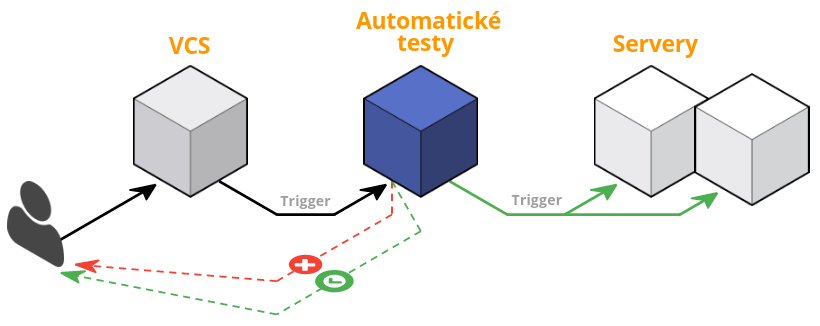
\includegraphics[width=\textwidth]{img/continuous-crop.png}}
	\caption{Continuous Integration}
	\small zdroj: Vlastní tvorba - \url{https://cloudcraft.co/}
	\label{fig:ci}
\end{figure}

Z~existujících testů se však dá těžit mnohem více. Automatické testy se hodí i při spolupráci více lidí, kdy je možné veškeré zaverzované změny na vzdáleném serveru okamžitě automaticky kontrolovat a v~případě, že aplikace funguje správně, můžeme spouštět například automatické nasazení nové verze aplikace na ostrý server (jako je to na obrázku \ref{fig:ci}). Zde platí, že čím více je kód pokryt testy, tím je menší šance na vznik nějaké chyby a je možné automatickým testům více věřit. Nemá smysl snažit se o~automatické nasazování nové verze na ostrý server, pokud testy nejsou, nebo je jich nedostatečně málo.

Podle obrázku \ref{fig:ci} programátor odesílá své kódy např. pomocí Gitu \cite{git} do vzdáleného repozitáře. Po odeslání se automaticky spouštějí testy a programátor tak získává zpětnou vazbu o~tom, jestli je vše stále funční či nikoliv. Celý proces může být složitější, ale základní myšlenka je pořád stejná. Důležité je mít pouze dostatečné pokrytí aplikace testy tak, aby se dalo testům důvěřovat, a pak je možné spoustu kroků zautomatizovat.

\subsection{Návrh databáze a databázové migrace}
Stejně tak jako se běžně verzují kódy aplikace, je třeba nějakým způsobem verzovat databázi. To je však (na rozdíl od kódu) velký problém. Verzování kódu totiž funguje stejně jako na obrázku \ref{fig:verzGit}. Pokud se kód nachází ve stavu A, tak naše změny představují rozdíl od této verze a po aplikování změn se dostáváme do dalšího stavu B. Důležité je, že v~každém kroku je kód jasně daný a tedy aplikujeme změny na známý stav.

\begin{figure}[h]
	\centering
	\makebox[\textwidth]{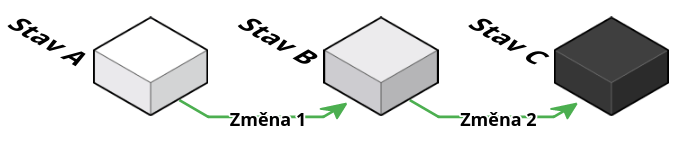
\includegraphics[width=\textwidth]{img/verzovani-git-crop.png}}
	\caption{Verzování kódu v~Gitu}
	\small zdroj: Vlastní tvorba - \url{https://cloudcraft.co/}
	\label{fig:verzGit}
\end{figure}

Změny databáze však fungují spíše podle obrázku \ref{fig:verzDb}. Databáze se neustále mění. Zejména pak její data, kvůli kterým je tento problém zcela odlišný od verzování kódu. Po aplikování změn totiž databáze nezůstane v~původním stavu. Vnitřní stav databáze se přirozeně mění a nový stav není nikdy přesně známý. Mění se z~toho důvodu, že uživatelé databázi používají - přidávají, mažou a aktualizují data. Takže zatímco v~kódu můžeme bez obav změny vracet, u~databáze to není možné a veškeré změny probíhají jen vpřed.

\begin{figure}[h]
	\centering
	\makebox[\textwidth]{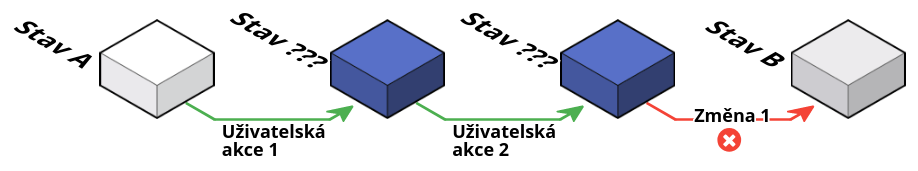
\includegraphics[width=\textwidth]{img/verzovani-db-crop.png}}
	\caption{Problém verzování databáze}
	\small zdroj: Vlastní tvorba - \url{https://cloudcraft.co/}
	\label{fig:verzDb}
\end{figure}

Z~toho důvodu je chytrou strategií vždy dělat zpětně kompatibilní změny. To znamená, že nově nasazená verze databáze vždy funguje i se starou verzí aplikace (z~hlediska aplikace je to dopředná kompatibilita). V~této práci jsou migrace zajišťovány pomocí knihovny Nextras Migrations \cite{nextras:migrations}. Tato knihovna zajišťuje kontrolu nad spouštěním databázových migrací ve správném pořadí. Je pak na programátorovi, aby nedělal destruktivní změny. Databázové migrace jsou v~adresářové struktuře uloženy takto:

\vspace{1em}
\dirtree{%
.1 migrations/.
.2 basic-data.
.3 2017.
.4 02.
.5 2017-02-03-104919-ws-series-ws3600.sql.
.2 dummy-data.
.3 2017.
.4 01.
.5 2017-01-31-091915-test-user.sql.
.4 02.
.5 2017-02-14-104504-weather-stations.sql.
.5 2017-02-23-161812-cameras.sql.
.2 structures.
.3 2017.
.4 01.
.5 2017-01-31-090810-initial.sql.
.4 02.
.5 2017-02-03-104848-ws-series.sql.
.5 2017-02-14-085713-ws-creation-date.sql.
.5 2017-02-15-095854-physical-quantities.sql.
.5 2017-02-21-155618-ws-record-creation-date.sql.
.5 2017-02-23-095726-cameras.sql.
}
\vspace{1em}

Jak je vidět, tak jsou změnové skripty označeny datem. Zároveň se v~databázi uchovává informace o~předchozích migracích. Při spuštění migrací přes CLI se tedy začnou provádět pouze zatím neaplikované změny a to v~pořadí podle času. Aplikace se tak dostane z~neznámého stavu do jiného neznámého stavu jasně definovanou cestou. Díky tomu, že jsou migrace součastí kódu, je možné je spouštět také v~průběhu automatického testování a nasazování nové verze aplikace na server.

\subsection{Zabezpečení API pro obousměrnou komunikaci}
Aby mohla klientská aplikace komunikovat se serverem, musí komunikovat prostřednictvím API. A~je naprosto nezbytné, aby tato klientská aplikace posílala autorizované požadavky. Jednak je nutné vědět, kdo požadavky posílá, a potom data, která server v~API nabízí, nejsou veřejně přístupná. V~této práci se využívá JW token (JWT) \cite{jwt}. Uživatel se nejdříve přes HTTPS přihlásí a po úspěšném ověření přihlašovacích údajů server vrátí JWT, který se uloží do \uv{local storage} v~prohlížeči. JWT vypadá takto:

\newcommand{\reducedstrut}{\vrule width 0pt height .9\ht\strutbox depth .9\dp\strutbox\relax}
\newcommand{\dotColor}[1]{%
  \begingroup
  \setlength{\fboxsep}{0pt}%  
  \colorbox{red}{\reducedstrut#1\/}%
  \endgroup
}
\begin{minted}[escapeinside=@@]{text}
eyJ0eXAiOiJKV1QiLCJhbGciOiJIUzUxMiJ9@\dotColor{.}@eyJpYXQiOjE0ODg3MzE5MDcsI
mV4cCI6MTQ4ODgxODMwNywidXVpZCI6IjAwMDAwMDAwLTAwMDAtMDAwMC0wMDA
wLTAwMDAwMDAwMDAwMSJ9@\dotColor{.}@odmV31XcAzVaKZpepNoSfnmavq3FDnZDFl2zhfR6
J54Yh8eFw2mj1Meq9nBUe5amtZRp45j9_xe8pIsJe7z7Jw
\end{minted}

Jedná se o~dlouhý řetězec, který obsahuje dvě tečky (barevně zvýrazněné). Tyto tečky dělí řetězec na další tři části. První část je zakódována pomocí base64 \cite{base64}, takže pro odhalení obsahu je možné použít funkci \texttt{atob} z~JavaScriptu:
%
\begin{minted}{javascript}
atob('eyJ0eXAiOiJKV1QiLCJhbGciOiJIUzUxMiJ9');
\end{minted}
%
Tato funkce vrátí JSON, který obsahuje informace o~tokenu, zejména pak o~použitém šifrovacím algoritmu:
%
\begin{minted}{javascript}
{"typ":"JWT","alg":"HS512"}
\end{minted}
%
Podobně je tomu i u~druhé části tokenu. Ta však navíc vrací libovolné informace, které si aplikace potřebuje předat:
%
\begin{minted}{javascript}
{
  "iat": 1488731907,
  "exp": 1488818307,
  "uuid": "00000000-0000-0000-0000-000000000001"
}
\end{minted}

V~tomto případě se jedná o~UUID uživatele, čas vystavení tokenu \texttt{iat} a čas expirace token \texttt{exp} (trvanlivost). Zatím se tedy jedná o~veřejně přístupné informace, které může kdokoliv získat. V~tokenu by neměla být žádná citlivá informace, protože uživatel (webový prohlížeč) pak tento token odesílá při každém požadavku a server ověřuje jeho pravost. Není tak nutné neustále posílat a někde uchovávat heslo. Aby nedošlo k~podvržení, tak token obsahuje ještě poslední část, která slouží jako ochrana proti napadení. K~vygenerování poslední části je nutné znát nejen data, ale i privátní klíč (v~předchozím příkladu je to slovo \texttt{secret}). Tímto privátním klíčem se token na serveru také ověřuje a pokud došlo ke změně informací v~tokenu, tak jej nepůjde ověřit a považuje se za nevalidní.

Webová aplikace posílá na server (resp. na API) HTTP požadavky s~hla\-vič\-kou \texttt{authorization}, která obsahuje JWT token. Tento způsob komunikace musí dodržet každý, kdo chce se serverem komunikovat. Server tak ví o~jakého uživatele se jedná a jestli je oprávněn danou operaci provést. Uživatel musí mít například přístup k~meteostanicím, ale jen k~těm, které vlastní.

%%%%%%%%%%%%%%%%%%%%%%%%%%%%%%%%%%%%%%%%%%%%%%%%%%

\section{Architektura uživatelského rozhraní}
Uživatelské rozhraní je napsáno s~pomocí React knihovny od společnosti Facebook \cite{reactjs}. Tato knihovna umí velmi dobře pracovat s~DOM v~prohlížeči pomocí deklarativního přístupu. To znamená, že odpovědností programátora je nadefinovat, jak by měl určitý stav aplikace vypadat a odpovědností React knihovny je co nejlepším způsobem se do tohoto stavu dostat\footnote{Opakem je imperativní programování. Zde programátor říká, co se má vykonávat. U~deklarativního programování naopak programátor říká, jak má vypadat koncový stav.}.

\subsection{Základy práce s~Reactem}
Celé uživatelské rozhraní se skládá z~komponent. Komponenty získávají data a podle těchto dat automaticky mění stav DOMu. Taková jednoduchá komponenta v~Reactu by mohla vypadat třeba takto:

\begin{minted}{jsx}
let Component = (props) =>
  <div className="fullname">
    I am {props.firstname}{' '}
    <strong>{props.surname}</strong>
  </div>;

ReactDOM.render(
  <Component firstname="John" surname="Doe"/>,
  document.getElementById('root')
);
\end{minted}

V~první části kódu je vytvořena komponenta s~názvem \texttt{Component} (\textbf{musí} začínat velkým písmenem), která obsahuje obyčejný \texttt{div} s~vypsáním jména a příjmení. Tyto hodnoty se dostanou do komponenty prostřednictvím tzv. vlastností (properties - props). Vlastnosti vždy přicházejí do komponenty zvenku, což je vidět v~druhé části kódu, kde se komponenta napojuje do DOMu. Zároveň jsou vlastnosti neměnné.

Tímto stylem je možné připravovat komponenty a pouze měnit jejich vlastnosti. React se postará o~správné vykreslení. Předchozí spuštěný kód vykreslí v~prohlížeči následující HTML:

\begin{minted}{html}
<div class="fullname">I am John <strong>Doe</strong></div>
\end{minted}

Možná to na první pohled nevypadá jako nic zajímavého. Dokonce se to může zdát jako příliš složité a nepraktické. Je třeba si však uvědomit, že taková komponenta lze použít na více místech a pouze změnou jejich vlastností ovládat výsledný stav. Navíc pracujeme jen s~minimálním HTML, takže je menší šance na vytvoření chyby. Celé uživatelské rozhraní se potom skládá z~drobných komponent (které se zase skládají z~jiných komponent) a tak vznikne výsledná stránka. Komponenty je také velmi jednoduché testovat.

Ačkoliv by se z~předchozích ukázek mohlo zdát, že se v~komponentě pracuje přímo s~HTML, tak to není pravda. Jedná se o~JSX. Tomu, co je JSX, je věnována celá následující sekce. Pro teď stačí, že předchozí kód je nutné ještě přeložit do čistého JavaScriptu, například pomocí nástroje Babel \cite{babel}. Díky tomu je možné používat moderní JavaScript ve starších prohlížečích. Výsledný kód pak vypadá takto:

\begin{minted}{javascript}
var Component = function Component(props) {
  return React.createElement(
    "div", { className: "fullname" },
    "I am ", props.firstname, ' ',
    React.createElement(
      "strong",
      null, // nemá žádné vlastnosti
      props.surname
    )
  );
};

ReactDOM.render(React.createElement(
  Component, { firstname: "John", surname: "Doe" }
), document.getElementById('root'));
\end{minted}

To je sice mnohem nepřehlednější kód, ale je zde hezky vidět, co se děje na pozadí. Každý element podobý HTML se ve skutečnosti překládání na volání funkce \texttt{createElement}, jejíž vstupní parametry jsou: název komponenty (elementu), její vlastnosti a výčet dalších elementů. Již na takto malé ukázce je vidět způsob zanořování komponent. To je také důvod, proč původní ukázka obsahuje mezeru za křestním jménem. Mezery se totiž zachovávají pouze pokud jsou v~řádce. Ostatní se zahazují a je třeba je pomocí JSX vynutit.

Existuje ještě jeden způsob komponent, které se vytváří pomocí tříd. Zde je ukázka stejné komponenty tímto novým způsobem:

\begin{minted}{jsx}
let Component = class extends React.Component {
  render = () =>
    <div className="fullname">
      I am {this.props.firstname}{' '}
      <strong>{this.props.surname}</strong>
    </div>;
};
\end{minted}

Způsob použití je stejný, výsledný kód je podobný, liší se pouze přístup k~vlastnostem. Tyto komponenty mají však navíc ještě tzv. stavy (anglicky states). To jsou vlastnosti komponenty, které jsou zapouzdřeny pouze v~jedné konkrétní komponentě a drží její vnitřní stav. Typicky se tak obsluhují třeba formuláře. Komponenta ví, co se s~formulářem děje a jak se mění, ale nikdo mimo komponentu k~této informaci nemá přístup.

Z~předchozích ukázek a vysvětlování by mělo být jasné, že data tečou skrz komponenty pouze směrem dolů od nadřazených komponent k~listům pomyslného grafu komponent. Ačkoliv je toto správný přístup, občas je potřeba ze zanořených komponent předávat informaci nadřazeným komponentám. Typickým zástupcem knihoven, které toto řeší, je Redux \cite{redux}. V~tomto případě již stav komponenty není uchován v~komponentě, ale v~globálním úložišti a veškeré změny stavu probíhají prostřednictvím tohoto úložiště. Zejména kvůli slovu \textit{globální} zní tento přístup jako slevení ze všech dobrých postupů, Redux je však mezi React vývojáři velmi oblíbený a v~této práci se hojně využívá.

\subsection{Dočasné Redux úložiště}
Díky tomu, že je React deklarativní, tak stačí někde udržovat stav aplikace a při jeho změně se potřebná část aplikace automaticky překreslí. Stav aplikace se běžně uchovává uvnitř každé komponenty. U~složitějších aplikací je však tento přístup spíše nevhodný, protože komponenty mohou předávat data pouze vnořeným komponentám a nikoliv nadřazeným. Redux \cite{redux} je knihovna, která se k~uchovávání stavu aplikace staví zcela jinak. Místo toho, aby se držel stav v~každé komponentě, tak si Redux pamatuje stav celé aplikace v~jednom úložišti. Díky tomu je možné v~průběhu životního cyklu aplikace postupně upravovat tento stav a React se postará o~překreslení DOMu.

Udržovat velké množství informací v~jednom úložišti může rychle přerůst programátorům přes hlavu. Redux proto obsahuje způsob, jak úložiště rozumným způsobem aktualizovat. Každá komponenta má možnost vytvořit a odeslat akci pomocí funkce \texttt{dispatch}. Redux se následně postará o~to, aby tato akce došla do tzv. reduceru, pokud nějaký existuje. Ten má za úkol příchozí akci nějakým způsobem zpracovat a aktualizovat úložiště (paměť). Následně dojde k~automatickému překreslení na všech místech, které tuto část paměti používají. Díky tomuto způsobu lze aktualizovat i nadřazené komponenty, jak je vidět na obrázku \ref{fig:redux}.

\begin{figure}[h]
	\centering
	\makebox[\textwidth]{\includegraphics[width=0.8\textwidth]{img/redux.png}}
	\caption{Aktualizace komponent prostřednictvím Reduxu}
	\label{fig:redux}
\end{figure}

Nadřazené komponenty by šlo aktualizovat i bez centrálního úložiště, horší případ by nastal u~komponent, které jsou ve stromu komponent na úplně jiném místě a nemají úzkou provázanost - přesto se nějak ovlivňují. Např. každá komponenta může vytvořit chybovou hlášku (také komponentu) napříč celou aplikací.

Akce jsou v~Reduxu obyčejné JavaScript objekty, pokud je však potřeba v~rámci akce spustit nějakou funkci (dotázat se API), je možné tak učinit. Pro akce, které nejsou jen objekty, je zapotřebí rozšiřujících knihoven jako je třeba Redux Thunk \cite{redux-thunk}. Reducer je potom úplně obyčejná funkce, která má k~dispozici původní stav úložiště a akci a na základě těchto informací vytváří novou podobu úložiště. Reducer by nikdy neměl měnit vstupní argumenty, ale vždy vrátit novou instanci, neměl by volat jiné funkce (data přicházejí v~akci) a měl by být deterministický (tzn. nepracovat s~datumem, náhodnými čísly, apod.).

Obrovskou výhodou je možnost řetězit jednotlivé akce případně rozkládat reducery. Spuštění akce nemusí znamenat jen jeden úkol, ale může spustit celou sekvenci akcí. Přidání nové meteostanice tak znamená zavolání API, ukázání průběhu zpracovávání, zobrazení zprávy o~úspěšném založení stanice a přesměrování - to vše vyvoláno jedním příkazem typu \uv{založ meteostanici s~názvem XY}.

Oproti uchovávání stavu uvnitř komponent je zde ještě jedna výhoda. Díky tomu, že jsou všechna data na jednom místě, je možné je uchovávat v~normalizované podobě a teoreticky tak ušetřit potřebné místo v~paměti.

\subsection{JSX}
V~roce 2009 byl poprvé zveřejněn projekt XHP jako open-source. Cílem bylo vytvořit způsob, jak eliminovat velké množství chyb a bezpečnostních problémů v~PHP \cite{hhvm:xhp}. Takže zatímco původní kód v~PHP pro vypsání krát\-ké\-ho HTML by vypadal takto:
%
\begin{minted}{text}
echo "<i>Hello <b>$user_name</b>!</i>";
\end{minted}
%
Tak v~XHP by stejný zápis vypadal následovně:
%
\begin{minted}{text}
echo <i>Hello <b>{$user_name}</b>!</i>;
\end{minted}
%
Na počet znaků se jedná o~stejné zápisy. Rozdíl je pouze v~uvozovkách a ve způsobu vypsání proměnné. Je zde však velký rozdíl ve významu. V~případě PHP se jedná pouze o~skládání řetězce, v~případě XHP se jedná o~celou gramatiku, která je součástí jazyka. Díky tomu bude v~případě XHP výstup vždy validní HTML a nebude obsahovat bezpečností chybu jako příklad s~PHP. Ten je náchylný na XSS útok.

XHP se překládá na PHP třídy reprezentující danou značku. Stejná my\-š\-len\-ka byla převzata do JavaScriptu ve formě JSX. Opět se HTML značky zapisují v~XML notaci a následně se překládají na jiný kód, který se stará o~stavbu DOMu a zabezpečení:

\begin{minted}{jsx}
let variable = 'class';
<div attribute={variable}>
  <Component/>
</div>
\end{minted}
%
Z~původního zápisu v~JSX se tak stane obyčejný JavaScript:
%
\begin{minted}{javascript}
var variable = 'class';
React.createElement(
  'div',
  { attribute: variable },
  React.createElement(Component, null)
);
\end{minted}

Aby se rozlišil obyčejný HTML tag a React komponenta, tak je nutné rozlišovat velikost počátečního písmena. Musí také existovat vždy jedna nad\-řa\-ze\-ná komponenta (stačí ve formě HTML):

\begin{minted}{html}
<div>
  <CapitalizedComponentName/>
  <justHtmlTag/>
</div>
\end{minted}
%
Z~výsledného přeloženého kódu bude jasné, proč tomu tak je:
%
\begin{minted}{javascript}
React.createElement(
  "div",
  null,
  React.createElement(CapitalizedComponentName, null),
  React.createElement("justHtmlTag", null)
);
\end{minted}

HTML tagy se překládají jako obyčejné řetězce, ale komponenty zůstávají jako proměnné. Takže aby předchozí kód fungoval, tak musí být někde dříve tato komponenta vytvořená, protože zde už je jen její použití, které v~případě JSX pouze vypadá hezky.

JSX je velmi intuitivní a veškeré možnosti jsou velmi dobře popsány v~dokumentaci \cite{jsx}. Proto si myslím, že je bezpředmětné psát do této práce to samé a raději bych se ještě zdržel u~jedné zvláštnosti, která má úzkou souvislost s~React vykreslováním DOMu a zaslouží si vysvětlení. Představme si následující kód:

\begin{minted}{jsx}
ReactDOM.render(
  <ul>
    {[1, 2, 3, 4, 5].map((item) =>
      <li>{item}</li>
    )}
  </ul>,
  document.getElementById('root')
);
\end{minted}

Sám o~sobě je tento kód naprosto v~pořádku. Vykreslí se bodový seznam pěti čísel. React si však bude stěžovat: \textit{Warning: Each child in an array or iterator should have a unique 'key' prop. Check the top-level render call using 'ul'.} Opravený kód podle chybové hlášky by vypadal takto:

\begin{minted}{jsx}
ReactDOM.render(
  <ul>
    {[1, 2, 3, 4, 5].map((item) =>
      <li key={item}>{item}</li>
    )}
  </ul>,
  document.getElementById('root')
);
\end{minted}

V~čem je problém? React totiž už při vykreslování ví, že pokud každá položka neobsahuje svůj jedinečný klíč, tak při změně dat v~určité situaci bude překreslení DOMu velmi výpočetně náročné. V~předchozím příkladu je v~seznamu pět čísel, ale těchto položek mohou být stovky. Pokud se tento výčet změní (například prostřednictvím vlastností komponenty), tak bude React hledat, kde je změna a na tomto místě aplikuje do DOMu opravu. Vymění se tak jen nutná část pro překreslení a původní položky zůstanou. To se stane i bez klíčů, pokud přidáme položku na konec seznamu.

Jenže existuje mnohem horší případ a tím je přidání položky na začátek seznamu. V~tom případě React porovná první položku a zjistí, že je DOM jiný. Druhá položka je však také jiná (protože se celý seznam posunul) a tak to jde dál až do konce. Je tedy nutné překreslit celý seznam. To je ale zbytečné kvůli jedné nové položce. Právě kvůli tomuto problému se používají klíče. Pokud je klíč unikátní, React může porovnat pouze klíče a snadno tak zjistí, že je nová položka na začátku seznamu. Překreslení je pak triviální.

Důležité je použít pro klíč nějakou hodnotu, která dostatečně dobře charakterizuje obsah HTML tagu. Je tedy nevhodné použít indexy pole, protože ty se mohou změnit (i když data ne). Stejně tak je nevhodné použít náhodnou hodnotu. Prakticky se pro tyto účely většinou používá ID z~databáze. V~před\-cho\-zí ukázce je to sama hodnota, to je však krajní případ.

\subsection{Komunikace se serverem pomocí GraphQL}
Všem komponentám z~předchozích ukázek je možné říkat prezentační komponenty. Tyto komponenty pouze prezentují (zobrazují) určitý stav na základě vstupů. Jedná se tedy o~naprosto předvídatelné komponenty, které v~mnoha případech nemusí mít ani vnitřní stav. Tímto stylem by však šlo napsat akorát statickou webovou stránku.

\begin{figure}[h]
	\centering
	\makebox[\textwidth]{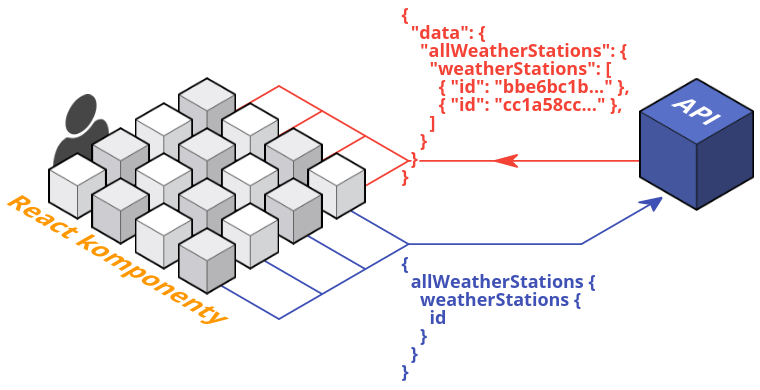
\includegraphics[width=\textwidth]{img/graphql-komunikace-crop.png}}
	\caption{GraphQL komunikace se serverem přes API}
	\small zdroj: Vlastní tvorba - \url{https://cloudcraft.co/}
	\label{fig:graphqlServer}
\end{figure}

Většinou je potřeba data někde získat. Od toho jsou nadřazené komponenty - tzv. kontejnery. Je nutné zdůraznit, že komponenta a kontejner je pořád to samé a píšou se stejně. Pro lepší návrh se však často rozlišuje jaké má komponenta závislosti. Takže pokud komponenta něco vykresluje, tak se stará \textbf{pouze} o~vykreslování a data získává pomocí vlastností. Pokud se komponenta stará o~získávání dat, tak jí říkáme kontejner (nebo nadřazená komponenta) a neměla by dělat nic jiného. V~této práci se pro komunikaci se serverem využívají asynchronní Redux akce \cite{redux}. Jak funguje Redux bylo podrobněji rozepsáno dříve. Nadřazené komponenty (kontejnery) pro komunikaci se serverem využívají GraphQL API. Toto API je vysvětleno podrobně později v~samostatné sekci.

Příkladem kontejneru je komponenta pro získání všech kamer, které jsou k~dispozici. Protože se tato komponenta nebude starat o~vykreslování, ale předá pouze data další komponentě na nižší úrovni, tak sama o~sobě není moc zajímavá. Zajímavější je její napojení do stromu komponent. Většinou je každá komponenta ve vlastním souboru a pouze se exportuje pro použití jinde. Kontejner je však ještě obalen do nadřazené komponenty, který ji připojuje do Redux úložiště. Díky tomu je pak možné spustit akci pro načtení všech kamer přesně v~okamžiku, kdy se komponenta připojuje do DOMu:

\begin{minted}{javascript}
export const AllCamerasContainer = class extends React.Component {

  componentWillMount() {
    this.props.dispatch(loadAllCameras()); // <-
  }

  render = () => { /* ... */ }
};

export default connect()(AllCamerasContainer);
\end{minted}

Tímto stylem se vlastně z~původní komponenty \texttt{AllCamerasContainer} stane ta samá komponenta, která již však (na rozdíl od původní) může pracovat s~Reduxem. Došlo tedy k~oddělení závislostí: kontejner získává data ze serveru a o~nic víc se již nestará. Naopak předává tyto data nějaké další komponentě. Tato prezentační komponenta je díky tomu velmi jednoduchá a hlavně jí nezáleží na původu dat. To se hodí i pro testování.

%%%%%%%%%%%%%%%%%%%%%%%%%%%%%%%%%%%%%%%%%%%%%%%%%%

\section{Architektura streamovací aplikace}
Streamovací aplikace slouží pouze pro zpracovávání obrazu z~kamer. Tato menší aplikace je naprogramována jako mikroslužba se kterou se komunikuje prostřednictvím jednoduchého API. Ačkoliv by mohl být tento kód součástí hlavního serveru, není tomu tak. Streamování totiž vyžaduje zcela jiné nároky na výpočetní výkon, a proto se vyplatí mít samostatný server, který se o~tento problém stará.

Ve svém jádru je tato aplikace velmi podobná hlavnímu serveru. Na rozdíl od něj je však naprogramována minimalisticky, takže je rychlá a moc toho neumí. Prakticky je možné pouze zapnout zpracování streamu a následně jej zase vypnout. Počítá se s~tím, že aplikace bude fungovat pouze v~rámci vnitřní sítě, takže není potřeba řešit ani žádné zabezpečení. Hlavní server jednoduše odešle na tuto službu požadavek na zpracování streamu a služba odpoví URL adresou, ze které je možné zpracované video přehrávat.

\subsection{Zapnutí a vypnutí zpracování streamu}
Vnitřně se hlavní aplikace ovládá pomocí příkazů, které vytvářejí nové zá\-zna\-my meteostanic nebo třeba nový záznam pro webovou kameru. Vytvářením je myšleno uložení nového záznamu do databáze. Právě tyto příkazy jsou vhodné místo pro vykonání dalších operací jako je třeba zapnutí konverze streamu videa. Server to dělá tak, že v~době ukládání informace o~nové kameře do databáze odesílá na streamovací server POST požadavek na zapnutí streamování. Vše probíhá v~jedné transakci, takže kdyby se náhodou nový stream na vzdálené službě nepodařilo zapnout, tak se ani v~databázi nevytvoří nová kamera.

Streamovací server má dvě URL adresy: \texttt{/startStream} a \texttt{/stopStream}. První zmíněná adresa očekává v~těle požadavku adresu původního streamu (tedy to, co nabízí webová kamera) a druhá adresa očekává ID streamu, který má být zastaven. Následuje ukázka zapnutí streamu pomocí příkazu \texttt{curl}, který umí POST požadavky posílat z~příkazové řádky \cite{curl}:

\begin{minted}{text}
curl --data "source=rtsp://stream.source" \
    http://stream.adeira.loc/startStream
\end{minted}

Streamovací aplikace odpoví ve formátu JSON, který obsahuje ID nového streamu (pro pozdější zastavení), dále původní adresu a hlavně novou adresu HLS playlistu. Ta je relativní, takže je možné měnit adresu tohoto serveru:

\begin{minted}{json}
{
  "data": {
    "id": "d736a5ff-7b91-4526-93cd-64c2fed230e8",
    "source": "rtsp:\/\/stream.source",
    "hls": "\/hls\/Y9c7gqdbevAzww7LfJYbJg\/stream.m3u8"
  }
}
\end{minted}
%
Obdobně funguje zastavování:
%
\begin{minted}{text}
curl --data "identifier=d736a5ff-7b91-4526-93cd-64c2fed230e8" http://stream.adeira.loc/stopStream
\end{minted}
%
Tentokrát se vrátí pouze ID smazaného streamu jako potvrzení úspěšné operace:
%
\begin{minted}{json}
{
  "data": {
    "identifier": "d736a5ff-7b91-4526-93cd-64c2fed230e8"
  }
}
\end{minted}

Tato aplikace si zachovává podobné chování jako hlavní server, takže pokud například dojde k~chybě, tak aplikace odpoví v~podobném JSON formátu, který obsahuje \texttt{error} pole:

\begin{minted}{json}
{
  "errors": [
    {
      "message": "Stream with identifier
                  'd736a5ff-7b91-4526-93cd-64c2fed230e8'
                  is not registered!"
    }
  ]
}
\end{minted}

Co se v~této aplikaci děje po přijetí požadavku na zpracování streamu? Aplikace obsahuje minimalistickou databázi SQLite \cite{sqlite}, do které se ukládají streamy pro zpracování. Na pozadí potom běží tolik procesů, kolik existuje zaregistrovaných streamů v~databázi. Jedná se o~procesy programu FFmpeg, jehož jediným úkolem je přijímat stream a překládat jej na HLS playlist a příslušné útržky videa.

%%%%%%%%%%%%%%%%%%%%%%%%%%%%%%%%%%%%%%%%%%%%%%%%%%

\section{Architektura konkretizačního uzlu}
Konkretizační uzel je jednoduchý program, který slouží pro převod uni\-kát\-ní\-ho formátu dat meteostanice na formát, kterému rozummí GraphQL API. Toto je jediné místo v~celém systému, kde existují konkrétní implementační detaily týkající se jedné konkrétní meteostanice. Cílem bylo, aby byl tento uzel co nejjednodušší. Pokud by byl potřebný program delší než několik desítek řádek kódu, nebyla by tato myšlenka moc použitelná. Implementace konkretizačního uzlu musí být pro koncového uživatele velmi jednoduchá. Jako příklad je zde uveden konkretizační člen stanice zmíněné v~úvodní části této práce.

Před samotným odesláním prvních dat je nutné získat JWT token pomocí přihlašovacího jména a hesla. K~tomu slouží jednoduchá \texttt{login} mutace, která se na server odešle jako POST požadavek:

\begin{minted}{graphql}
mutation {
  login (username: "user", password: "pass") {
    token
  }
}
\end{minted}

Tomu co znamenají jednotlivé části dotazu se podrobně věnuje následující kapitola. Důležité je, že server odpoví JWT tokenem, který se používá pro ověřování následujících odesílaných požadavků. Tento token je možné někam dočasně uložit, protože jeho expirace chvíli trvá. Ničemu však nevadí získat pokaždé nový token. Jen je nutné ptát se přes zabezpečené HTTPS spojení.

Nyní zbývá odeslat nějaká data na server prostřednictvím POST po\-ža\-dav\-ku. Tato meteorologická stanice má bohužel jedno specifikum. Kromě počítače, který je připojený přímo, neumí data nikam odesílat. Konkretizační uzel by mohl běžet na nějakém vzdáleném serveru, ale v~tomto případě musí být puštěn přímo na počítači u~meteostanice. Zde vždy získá poslední záznam ze souboru \texttt{history.dat} a odešle jej přes GraphQL API na server. Data se opět odesílají díky mutaci, jejíž vstupní data mají tuto podobu:

\begin{minted}{javascript}
{
  id: '00000000-0001-0000-0000-000000000001',
  input: {
    absolutePressure: 966.4,
    relativePressure: 1006.4,
    indoorTemperature: 24.4,
    outdoorTemperature: null,
    indoorHumidity: 32,
    outdoorHumidity: null,
    windSpeed: null,
    windAzimuth: null,
    windGust: null,
    pressureUnit: 'PASCAL',
    humidityUnit: 'PERCENTAGE',
    windSpeedUnit: 'KMH',
    temperatureUnit: 'CELSIUS'
  }
}
\end{minted}

Z~ukázky je vidět, že meteostanice neumí všechny fyzikální veličiny. Chy\-bě\-jí\-cí položky je možné odeslat s~hodnotou \texttt{null}, nebo je úplně vypustit. Asi nejzajímavější částí jsou jednotky jednotlivých fyzikálních veličin. Hlavní server totiž umí velmi dobře pracovat s~jednotkami a interně provádí přepočty podle potřeby. V~současné době je možné použít tyto jednotky:

\begin{itemize}
\item tlak: pascal, bar, torr, fyzikální atmosféra
\item teplota: Celsius, Fahrenheit, Kelvin
\item vlhkost: procento
\item rychlost: km/h, míle/h, m/s
\end{itemize}

Tyto jednotky není potřeba přes API odesílat, pokud se jednotky jednotlivých hodnot neliší od výchozích. Předchozí data by tedy bylo možné zjednodušit takto:

\begin{minted}{javascript}
{
  id: '00000000-0001-0000-0000-000000000001',
  input: {
    absolutePressure: 966.4,
    relativePressure: 1006.4,
    indoorTemperature: 24.4,
    indoorHumidity: 32
  }
}
\end{minted}

Význam je stejný. Samozřejmě platí, že odesílaná data jsou v~JSON formátu a je tedy možné z~požadavku odstranit bílé znaky. Zde jsou ukázky rozepsány pouze pro přehlednost. Na rychlost by to zde nemělo žádný zásadní vliv, v~praxi se však ukazuje, že odpovědi ze serveru je vhodné takto minifikovat, protože velikost přenášených dat může klesnout až na polovinu\footnote{Prakticky ověřeno na odpovědi vrácené z~GraphQL API společnosti Kiwi.com. Původní odpověď o~velikosti 522 KB se odstraněním bílých znaků zmenšila na 266 KB.}.

Slovo architektura je v~případě konkretizačního uzlu až příliš nadnesené. V~součtu má program asi 100 řádek kódu a většina je pouze definice binárního formátu dat. Kód, který něco skutečně vykonává má jen asi 20 řádek. Bez okolního kontextu by však nedával smysl (protože využívá externí knihovny) a je proto k~dispozici na elektronickém médiu, které je přiloženo k~této závěrečné práci.

%%%%%%%%%%%%%%%%%%%%%%%%%%%%%%%%%%%%%%%%%%%%%%%%%%

\section{GraphQL API}
GraphQL \cite{graphql} je API, které bylo vynalezeno společností Facebook pro chy\-třej\-ší komunikaci klientských částí se serverem. Jeho velkou předností je, že se jedná o~dotazovací jazyk. Je tedy možné doptat se serveru na libovolnou podmnožinu dat. To je rozdíl například oproti REST API (nebo téměř ja\-ké\-mu\-ko\-liv jinému API). Většinou je totiž API navržené tak, že nabízí jasně definované koncové body na které se uživatel může ptát. Z~těchto bodů se také většinou vrací jasně definovaná data. GraphQL ale funguje úplně jinak.

GraphQL API nabízí pouze jednu URL adresu, na kterou je možné posílat dotazy. To je zpravidla adresa \texttt{/graphql}. Na tuto adresu se posílají POST HTTP požadavky. Tělo těchto požadavků pak nese informaci o~tom, jaká data chceme získat. Tato informace může být téměř libovolná. Na straně serveru se pak vytvoří graf všech dat, která jsou v~API k~dispozici. Jako příklad uveďme jednoduchý dotaz na seznam všech meteorologických stanic. Klient pošle POST požadavek na server v~tomto znění (zjednodušeno):

\begin{minted}{text}
POST /graphql HTTP/1.1
Host: connector.adeira.loc
Connection: keep-alive
Content-Length: 91
accept: application/json
content-type: application/json
Accept-Encoding: gzip, deflate
Accept-Language: en-US,en;q=0.8
\end{minted}
%
Tělo požadavku obsahuje následující JSON data:
%
\begin{minted}{json}
{
  "query": "{allWeatherStations{weatherStations{id}}}",
  "variables": null,
  "operationName": null
}
\end{minted}

Za povšimnutí stojí hodnota \texttt{query}, která obsahuje GraphQL dotaz. Ten má vlastní zápis, který na první pohled vypadá jako zjednodušený JSON:

\begin{minted}{graphql}
{
  allWeatherStations {
    weatherStations {
      id
    }
  }
}
\end{minted}

V~tomto dotazu se ptáme na všechny meteorologické stanice a u~těchto stanic nás zajímá pouze jejich identifikátor. Server následně odpoví ná\-vra\-to\-vým kódem \texttt{HTTP/1.1 200 OK} a společně s~hlavičkami pošle požadovaná data:

\begin{minted}{json}
{
  "data": {
    "allWeatherStations": {
      "weatherStations": [
        { "id": "bbe6bc1b-386f-4b6d-91e4-379c7882792c" },
        { "id": "cc1a58cc-1fd9-46f9-a193-d7e942a01019" }
      ]
    }
  }
}
\end{minted}

Z~této krátké ukázky by měla být vidět obrovská výhoda GraphQL. Data totiž nějsou nijak vázána na URL adresu, ale výběr požadovaných dat se provádí popsáním podmnožiny grafu, který nás zajímá. Ten je poslán jako tělo POST požadavku, takže se může kdykoliv libovolně měnit a podle toho se změní také odpověď.

Předchozí ukázka obsahuje pouze dotazování se na data. To by však bylo pro API málo. Server je potřeba i ovládat a od toho jsou zde mutace. Tyto dvě hlavní skupiny jsou kromě dalších vlastností API popsány dále.

\subsection{Typy (Types)}
Aby bylo možné získávat z~API nějaká data, je potřeba definovat tzv. typy. Ty formují strukturu navrácených dat. Předchozí příklad s~dotazem na všechny indentifikátory meteostanic obsahoval tři typy. Ty sice na první pohled nejsou vidět, ale pomocí nich je API nadefinováno. Předpis těchto typů by vypadal následovně:

\begin{minted}{graphql}
type Query {
  allWeatherStations: WeatherStationsConnection
}

type WeatherStationsConnection {
  totalCount: Int!
  weatherStations: [WeatherStation]
}

type WeatherStation {
  id: ID!
  name: String!
}
\end{minted}

Tyto typy toho obsahují ve skutečnosti více, ale pro pochopení to pro teď stačí. První typ \texttt{Query} definuje sadu všech dotazů, které můžeme položit. Pokud se zeptáme jako v~předchozím případě na všechny meteostanice, tak dostaneme \texttt{Connection} typ. Na této úrovni můžeme doplnit nějaké další potřebné informace, jako je celkový počet dostupných stanic a samozřejmě samotné stanice. Vykřičník v~návratové hodnotě značí povinnou položku. Konečně dotazem na typ meteostanice můžeme získat ID stanice nebo třeba její jméno. Všechny typy jsou k~dispozici v~interaktivní dokumentaci API, takže sestavit správný dotaz není složité.

\subsection{Dotazy (Queries)}
Již v~předchozích ukázkách byl použit jednoduchý dotaz pro získání ID všech meteostanic. Tyto dotazy umoňují získat z~API téměř libovolnou informaci. Jednou z~nejužitečnějších vlastností jsou argumenty dotazu. Zatímco vytažení všech meteostanic nepotřebuje žádné argumenty, tak pokud chceme pouze jednu konkrétní stanici, musíme specifikovat jakou. To jde v~GraphQL udělat třeba takto:

\begin{minted}{graphql}
{
  weatherStation(id: "bbe6bc1b-386f-4b6d-91e4-379c7882792c") {
    id
    name
  }
}
\end{minted}
%
Odpověď je opět JSON obsahující dotázané informace (ID a název). Uži\-teč\-nost argumentů je pak ještě lépe vidět ve spojení s~proměnnými. 
%
\begin{minted}{graphql}
query ($id: ID!) {
  weatherStation(id: $id) {
    id
    name
  }
}
\end{minted}

Toto je plnohodnotný zápis dotazu a lze jednoduše použít jako takový předpis pro jeden typ dotazů. Souběžně s~tímto dotazem se totiž posílá i JSON, který obsahuje ID. Toto ID se může libovolně měnit a dotaz zůstává pořád stejný.

Další příjemnou vlastností je možnost zeptat se na více věcí najednou:

\begin{minted}{graphql}
query ($stationId: ID!, $userId: ID!) {
  weatherStation(id: $stationId) {
    id
    name
  }
  user(id: $userId) {
    id
    username
    token
  }
}
\end{minted}

Opět je nutné poslat souběžně hodnoty proměnných a opět se vrátí JSON obsahující požadovaná data. GraphQL je velmi intuitivní a díky interaktivní dokumentaci API je pokládání dotazů velmi jednoduché a dokonce i s~napovídáním.

Díky tomu, že se API skutečně chová jako graf, tak je možné pokládat dokonce rekurzivně zanořené dotazy (uživatel vlastní meteostanice, kde každá meteostanice je vlastněna nějakým uživatelem, kde každý uživatel vlastní nějaké meteostanice...). Proto je nutné na serveru dávat pozor na přílišnou složitost položeného dotazu a případně odpovědět chybou.

\subsection{Mutace (Mutations)}
Podobně jako dotazy získávají ze serveru data, tak mutace data na serveru mění. Zároveň však data stejně jako dotazy získávají. Rozdíl je pouze v~tom, že mutace mají trošku jiný zápis a mohou něco změnit. Navíc mutace jsou zpracovávány sériově, kdežto dotazy mohou být na serveru pracovány souběžně (nehrozí kolize). Příkladem velmi jednoduché mutace je přihlašování:

\begin{minted}{graphql}
mutation {
  login(username: "test", password: "test") {
    id
    username
    token
  }
}
\end{minted}

Je vidět, že vnitřek dotazu je stejný jako u~\uv{queries}. Dotaz však začíná klíčovým slovem \texttt{mutation} a volá nějakou konkrétní mutaci (zde \texttt{login}). Server v~případě úspěšného přihlášení odpovídá mimo jiné JWT tokenem, který je dále používán pro ověřování místo přihlašovacího jména a hesla. O~něco složitější mutace je potřeba pro vytvoření nového záznamu meteostanice:

\begin{minted}{graphql}
mutation create(
  $stationId: ID!, $quantities: PhysicalQuantitiesInput!
) {
  createWeatherStationRecord(
    id: $stationId, quantities: $quantities
  ) {
    id, creationDate
  }
}
\end{minted}

Jak je vidět, tak v~argumentech není nutné posílat pouze skalární hodnoty, ale je možné poslat celý objekt. Ten musí být vždy odeslán souběžně ve formátu JSON. Pro předchozí mutaci by tělo požadavku mohlo vypadat třeba takto:

\begin{minted}{json}
{
  "stationId": "00000000-0001-0000-0000-000000000001",
  "quantities": {
    "absolutePressure": 100000,
    "relativePressure": 100000,
    "pressureUnit": "PASCAL"
  }
}
\end{minted}
%
Návratová hodnota ze serveru je také ve formátu JSON a obsahuje ID nového záznamu a čas vytvoření tohoto záznamu:
%
\begin{minted}{json}
{
  "data": {
    "createWeatherStationRecord": {
      "id": "4b9126b3-cbed-4a63-9acf-49a61f6a9fc0",
      "creationDate": "2017-03-12T14:37:31+01:00"
    }
  }
}
\end{minted}

Mutace jsou velmi podobné dotazům. Stačí pouze pochopit jak fungují dotazy a uvědomit si, že mutace mohou měnit stav aplikace. Pomocí těchto dvou jednoduchých metod je možné vykonat jakoukoliv myslitelnou operaci, kterou API umoňuje. To je vlastně také hlavní myšlenka celé serverové aplikace - poskytnout dostatečně mocné API a žádné uživatelské rozhraní.

\subsection{Stránkování v~GraphQL}
Stránkování je speciální požadavek na API, který jde mimo všechny ostatní. Můžeme například chtít získávat meteostanice po deseti tak, aby bylo možné vytvořit jednotlivé stránky s~jejich kratším přehledem. Podobně jako se to dělá na internetových obchodech pro stránkování produktů. Přitom většina API je postavená tak, že zobrazí jeden záznam nebo všechny záznamy. Jak si s~tímto problémem poradit? Řešením jsou uzly a hrany grafu:

\begin{minted}{graphql}
query paginateStations {
  allWeatherStations(first: 10) {
    totalCount
    edges {
      cursor
      node {
        id # konkrétní meteostanice
      }
    }
  }
}
\end{minted}

Takto lze získat prvních deset meteostanic. Je vidět, že samotné tělo dotazu je mnohem složitější než obvykle. Na první úrovni jsou hrany grafu (edges) a jejich celkový počet. Celkový počet hran je zároveň celkový počet meteostanic. Každá hrana následně obsahuje kurzor a uzel grafu. Uzel grafu obsahuje jednotlivé položky meteostanice, které nás zajímají. Kurzor potom představuje ukazatel na konkrétní hranu grafu. Skvělé na tomto návrhu je to, že získáme požadovaných deset meteostanic a zároveň víme jejich celkový počet a známe kurzor poslední hrany (např. \texttt{CUr50r}), takže dotaz na dalších deset meteostanic je velmi přímočarý:

\begin{minted}{graphql}
query paginateStations {
  allWeatherStations(first: 10, after: "CUr50r") {
    totalCount
    edges {
      cursor
      node {
        id # konkrétní meteostanice
      }
    }
  }
}
\end{minted}

Existuje více způsobů jak pracovat se stránkováním a i předchozí způsob je nutné pomocí GraphQL vytvořit. Je tedy na programátorovi jaký způsob zvolí. Kurzorový přístup se však velmi osvědčil a pro GraphQL API je vhod\-ným kandidátem. Může se zdát, že je to až příliš složité, ale pokud si uvě\-do\-mí\-me, kolik informací lze jedním dotazem získat, tak to za tu námahu stojí.

\subsection{Pokročilé možnosti GraphQL}
Všechny dříve popsané možnosti GraphQL API plně dostačují pro téměř jakýkoliv požadavek. Existuje však celá řada vylepšení a pomůcek, které umožňují pokládané dotazy zpřehlednit, případně doplnit o~nějaké další vlast\-nosti. Následuje krátký výčet těchto pokročilých možností, který je zde uveden spíše pro úplnost.

\subsubsection{Aliasy}
Pomocí aliasů lze změnit názvy jednotlivých hodnot, které API vrací. Aliasy se uvádějí před výraz a končí dvojtečkou:

\begin{minted}{graphql}
query getName {
  uzivatel: user(id: "00000000-0000-0000-0000-000000000001") {
    jmeno: username
  }
}
\end{minted}
%
Původní dotaz by vrátil odpověď obsahující slova \textit{user} a \textit{username}. Nově však vrátí jejich české varianty:
%
\begin{minted}{json}
{
  "data": {
    "uzivatel": {
      "jmeno": "John Doe"
    }
  }
}
\end{minted}

\subsubsection{Fragmenty}
Některé dotazy mohou být velmi složité a může se stát, že se některé části dotazu budou opakovat. V~GraphQL si lze ušetřit práci pomocí fragmentů. Každý fragment obsahuje výčet polí nad určitým typem a tento fragment lze používat na více místech. Fragmenty se uplatní až u~rozsáhlejších dotazů, ale pro ukázku zápisu následuje jednoduchý příklad:

\begin{minted}{graphql}
query getUserInfo {
  user(id: "00000000-0000-0000-0000-000000000001") {
    ...UserFields
  }
}

fragment UserFields on User {
  id, username, token
}
\end{minted}

Jak lze očekávat, tak API vrátí ID uživatele, jeho uživatelské jméno a JWT token. Pokud by bylo potřeba získat v~jiné části dotazu ta stejná data, tak je možné volání fragmentu opakovat. Fragment lze také zapsat jako součást dotazu:

\begin{minted}{graphql}
query getUserInfo {
  user(id: "00000000-0000-0000-0000-000000000001") {
    ... on User {
      id, username, token
    }
  }
}
\end{minted}

V~tomto jednoduchém příkladu to však nedává smysl, protože stejného efektu lze dosáhnout i bez fragmentu. Tato varianta se hodí pouze v~případě, že by daný uzel grafu vracel více typů. Pak je možné na základě typu pracovat s~jinými hodnotami. Ve spojení s~aliasy to umožnuje pokládat poměrně zajímavé dotazy.

\subsubsection{Direktivy}
Pomocí direktiv lze podmiňovat, případně jinak měnit chování položeného dotazu:

\begin{minted}{graphql}
query getUsernameOrToken($switch: Boolean!) {
  user(id: "00000000-0000-0000-0000-000000000001") {
    username @skip(if: $switch)
    token @include(if: $switch)
  }
}
\end{minted}
% $

Tento příklad ukazuje dvě vestavěné direktivy podle specifikace. Pomocí přepínače je tak možné získat uživatelské jméno nebo token, ale ne obojí najednou. Díky tomu je možné vytvořit složité dotazy a podmiňovat, jestli chceme úplný výběr nebo jen podvýběr. Tyto direktivy je možné přidávat i vlastní. Zde je však nutné se nejdříve zamyslet, jestli je to skutečně nutné.

\subsubsection{Introspekce}
Nástroje jako GraphiQL \cite{graphiql} umí zobrazit celé schéma API a napovídají jeho možnosti při psaní dotazu. Jak je to ale možné? Jak tento nástroj sám od sebe ví, co API umí? K~tomu slouží tzv. introspekce. GraphQL totiž nabízí možnost, jak API prozkoumávat a zjišťovat potřebné podrobnosti. Princip je pořád stejný, jen tyto systémové typy začínají dvojicí podtržítek:

\begin{minted}{graphql}
{
  __schema {
    directives {
      name, description, locations
      args { name, description }
    }
  }
}
\end{minted}

Tímto dotazem lze například získat informace o~dříve použitých direktivách - jejich názvy, popis funkce, kde je lze použít a jaké mají argumenty. Stejným způsobem je možné zeptat se na téměř cokoliv. Celé API je tedy velmi transparentní a samo sobě dělá jednoduchou dokumentaci.

\subsection{Chybové stavy v~GraphQL}
V~průběhu pokládání dotazů se může stát, že vznikne nějaká chyba. Chyby vznikají a není potřeba se jich bát, ale zejména v~API je s~nimi potřeba dobře zacházet. To znamená, že úspěšná odpověď je pouze tehdy, pokud server vrátí HTTP kód 200. Cokoliv jiného je pravděpodobně známka chyby. V~GraphQL mohou nastat tři hlavní chybové stavy. První je \uv{syntax error}, pokud uživatel odešle na server nevalidní formát dotazu. Kromě toho, že server odpoví kódem 422, tak odešle také JSON popisující, kde je problém:

\begin{minted}{json}
{
  "errors": [
    {
      "message": "
Syntax Error (1:14) Expected :, found String \"User\"
1: {__type(name \"User\"){kind}}
                ^",
      "locations": [
        { "line": 1, "column": 14 }
      ]
    }
  ]
}
\end{minted}

Odpověď je ve formátu JSON, takže může působit na první pohled ne\-pře\-hled\-ně, ale hned v~zápětí je vidět jaký dotaz byl odeslán a kde je chyba. Toto je důvod, proč jsou vrácená data z~tohoto API vždy zanořena v~klíči \texttt{data}. Chyby se totiž posílají s~klíčem \texttt{errors}. Podobně může vzniknout validační chyba, kde je sice dotaz zapsán správně, ale nesplňuje předem dané požadavky. Příkladem může být hodnota s~jiným datovým typem v~argumentu, než je očekáván: \texttt{Argument 'name' got invalid value User. Expected type 'String', found User.}

Posledním příkladem je vnitřní chyba serveru. V~tomto případě je dotaz validní a správný, ale server selhal a proto vrací pole errorů jako v~předchozím příkladu, ale navíc i pole dat s~\texttt{NULL} hodnotami na místě selhání:

\begin{minted}{json}
{
  "data": null,
  "errors": [
    {
      "message": "Internal Server Error."
    }
  ]
}
\end{minted}

Nyní je na uživateli tohoto API, aby se k~takovým chybám náležitě zachoval. Může je zobrazit uživateli ve webové aplikaci, nebo je tiše ignorovat. Záleží na konkrétním případu.